\section{Stream}
Aquest benchmark es centra en testejar el bandwidth a memòria.
Es composa de 4 funcions: \texttt{Copy}, \texttt{Scale}, \texttt{Add} i \texttt{Triad}.
La funció que fa només operacions a memoria és la de \texttt{copy}, per tant ens serveix per a fer la línia de memòria en un \textit{roofline} amb dades empíriques i no teòriques.

\subsection{One-node performance}


\begin{table}[h]
    \centering
\begin{tabular}{cccc}
Processes            & Function                     & Best Rate Bandwidth (MB/s)                              & Avg time (s)                 \\ \hline \hline
                     & \cellcolor[HTML]{EFEFEF}Copy & \cellcolor[HTML]{EFEFEF}{\color[HTML]{000000} 1.44E+04} & \cellcolor[HTML]{EFEFEF}0.10 \\
                     & Scale                        & {\color[HTML]{000000} 8.64E+03}                         & 0.14                         \\
                     & \cellcolor[HTML]{EFEFEF}Add  & \cellcolor[HTML]{EFEFEF}{\color[HTML]{000000} 9.28E+03} & \cellcolor[HTML]{EFEFEF}0.22 \\
\multirow{-4}{*}{1}  & Triad                        & {\color[HTML]{000000} 9.31E+03}                         & 0.17                         \\ \hline
                     & \cellcolor[HTML]{EFEFEF}Copy & \cellcolor[HTML]{EFEFEF}{\color[HTML]{000000} 2.84E+04} & \cellcolor[HTML]{EFEFEF}0.06 \\
                     & Scale                        & {\color[HTML]{000000} 1.71E+04}                         & 0.08                         \\
                     & \cellcolor[HTML]{EFEFEF}Add  & \cellcolor[HTML]{EFEFEF}{\color[HTML]{000000} 1.83E+04} & \cellcolor[HTML]{EFEFEF}0.12 \\
\multirow{-4}{*}{2}  & Triad                        & {\color[HTML]{000000} 1.83E+04}                         & 0.12                         \\ \hline
                     & \cellcolor[HTML]{EFEFEF}Copy & \cellcolor[HTML]{EFEFEF}{\color[HTML]{000000} 4.13E+04} & \cellcolor[HTML]{EFEFEF}0.04 \\
                     & Scale                        & {\color[HTML]{000000} 2.76E+04}                         & 0.06                         \\
                     & \cellcolor[HTML]{EFEFEF}Add  & \cellcolor[HTML]{EFEFEF}{\color[HTML]{000000} 3.01E+04} & \cellcolor[HTML]{EFEFEF}0.07 \\
\multirow{-4}{*}{4}  & Triad                        & {\color[HTML]{000000} 3.02E+04}                         & 0.07                         \\ \hline
                     & \cellcolor[HTML]{EFEFEF}Copy & \cellcolor[HTML]{EFEFEF}{\color[HTML]{000000} 3.83E+04} & \cellcolor[HTML]{EFEFEF}0.05 \\
                     & Scale                        & {\color[HTML]{000000} 2.90E+04}                         & 0.05                         \\
                     & \cellcolor[HTML]{EFEFEF}Add  & \cellcolor[HTML]{EFEFEF}{\color[HTML]{000000} 3.28E+04} & \cellcolor[HTML]{EFEFEF}0.07 \\
\multirow{-4}{*}{8}  & Triad                        & {\color[HTML]{000000} 3.35E+04}                         & 0.06                         \\ \hline
                     & \cellcolor[HTML]{EFEFEF}Copy & \cellcolor[HTML]{EFEFEF}{\color[HTML]{000000} 4.69E+04} & \cellcolor[HTML]{EFEFEF}0.02 \\
                     & Scale                        & {\color[HTML]{000000} 3.41E+04}                         & 0.03                         \\
                     & \cellcolor[HTML]{EFEFEF}Add  & \cellcolor[HTML]{EFEFEF}{\color[HTML]{000000} 3.81E+04} & \cellcolor[HTML]{EFEFEF}0.04 \\
\multirow{-4}{*}{16} & Triad                        & {\color[HTML]{000000} 3.84E+04}                         & 0.04                         \\ \hline 
\end{tabular}
    \caption{Performance en MB/s i temps de cada funció amb diferent nombre de processos.}
    \label{tab:stream_nobinding_perf}
\end{table}

\begin{figure}[h]
    \centering
    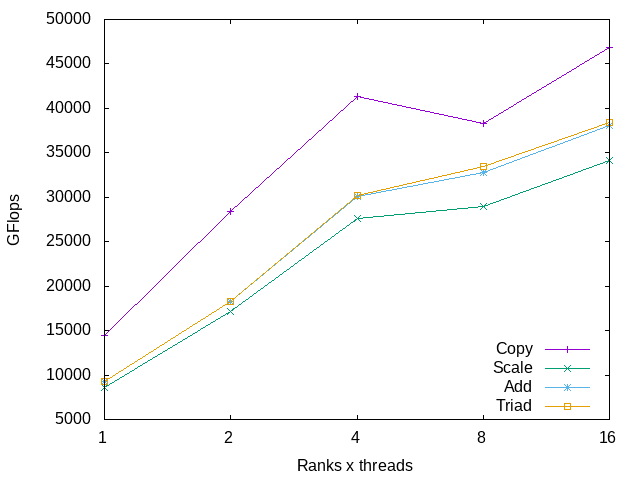
\includegraphics[width=0.5\textwidth]{img/stream_nobinding_grafica.png}
    \caption{Gràfica amb la performance de MB/s mitjana per diferent nombre de processos.}
    \label{fig:stream_nobinding_perf}
\end{figure}

Observant els resultats de bandwidth de la funció \texttt{Copy}, ja que es l'única que té operacions estrictament a memòria, veiem que es va satura a partir de 4 threads.

\subsection{Peak memory bandwidth}

Bandwidth teòric de DDR4-2400:

\[2400\ transfers/s\ *\ (64\ bits/8\ bits/byte)\ *\ 6\ channels\ =\ 115.20\ MB/s\]

Bandwidth teòric de DDR4-2133:

\[2133\ transfers/s\ *\ (64\ bits/8\ bits/byte)\ *\ 6\ channels\ =\ 102.38\ MB/s\]

Per poder realitzar una bona comparativa, hauriem d'haver executat el benchmark també amb 6 i 12 threads.
Així podríem comparar exactament el bandwidth obtingut al tenir tants threads com canals a memòria.

Crec que he calculat malament el bandwidth teòric perquè es inferior al bandwidth reportat per Stream.


\subsection{Numactl}
Com veiem a la taula \ref{tab:stream_binding_same_perf} i la gràfica \ref{fig:stream_binding_one_same_perf}, a partir de 4 threads no escala, es satura el bandwith
\begin{table}[h]
    \centering
\begin{tabular}{cccc}
Processes            & Function                     & Best Rate (MB/s)                 & Avg time (s)                 \\ \hline \hline
                     & \cellcolor[HTML]{EFEFEF}Copy & \cellcolor[HTML]{EFEFEF}1.42E+04 & \cellcolor[HTML]{EFEFEF}0.07 \\
                     & Scale                        & 8.53E+03                         & 0.11                         \\
                     & \cellcolor[HTML]{EFEFEF}Add  & \cellcolor[HTML]{EFEFEF}9.19E+03 & \cellcolor[HTML]{EFEFEF}0.16 \\
\multirow{-4}{*}{1}  & Triad                        & 9.18E+03                         & 0.16                         \\ \hline
                     & \cellcolor[HTML]{EFEFEF}Copy & \cellcolor[HTML]{EFEFEF}2.30E+04 & \cellcolor[HTML]{EFEFEF}0.04 \\
                     & Scale                        & 1.42E+04                         & 0.07                         \\
                     & \cellcolor[HTML]{EFEFEF}Add  & \cellcolor[HTML]{EFEFEF}1.56E+04 & \cellcolor[HTML]{EFEFEF}0.09 \\
\multirow{-4}{*}{2}  & Triad                        & 1.56E+04                         & 0.09                         \\ \hline
                     & \cellcolor[HTML]{EFEFEF}Copy & \cellcolor[HTML]{EFEFEF}2.49E+04 & \cellcolor[HTML]{EFEFEF}0.04 \\
                     & Scale                        & 1.72E+04                         & 0.06                         \\
                     & \cellcolor[HTML]{EFEFEF}Add  & \cellcolor[HTML]{EFEFEF}1.96E+04 & \cellcolor[HTML]{EFEFEF}0.07 \\
\multirow{-4}{*}{4}  & Triad                        & 1.95E+04                         & 0.07                         \\ \hline
                     & \cellcolor[HTML]{EFEFEF}Copy & \cellcolor[HTML]{EFEFEF}2.42E+04 & \cellcolor[HTML]{EFEFEF}0.04 \\
                     & Scale                        & 1.70E+04                         & 0.06                         \\
                     & \cellcolor[HTML]{EFEFEF}Add  & \cellcolor[HTML]{EFEFEF}1.94E+04 & \cellcolor[HTML]{EFEFEF}0.07 \\
\multirow{-4}{*}{8}  & Triad                        & 1.94E+04                         & 0.07                         \\ \hline
                     & \cellcolor[HTML]{EFEFEF}Copy & \cellcolor[HTML]{EFEFEF}2.44E+04 & \cellcolor[HTML]{EFEFEF}0.04 \\
                     & Scale                        & 1.73E+04                         & 0.06                         \\
                     & \cellcolor[HTML]{EFEFEF}Add  & \cellcolor[HTML]{EFEFEF}1.96E+04 & \cellcolor[HTML]{EFEFEF}0.07 \\
\multirow{-4}{*}{16} & Triad                        & 1.96E+04                         & 0.07                         \\ \hline
\end{tabular}
    \caption{Performance en MB/s i temps de cada funció amb diferent nombre de processos en un mateix numanode tant la memòria com els processos.}
    \label{tab:stream_binding_same_perf}
\end{table}

\begin{figure}[h]
    \centering
    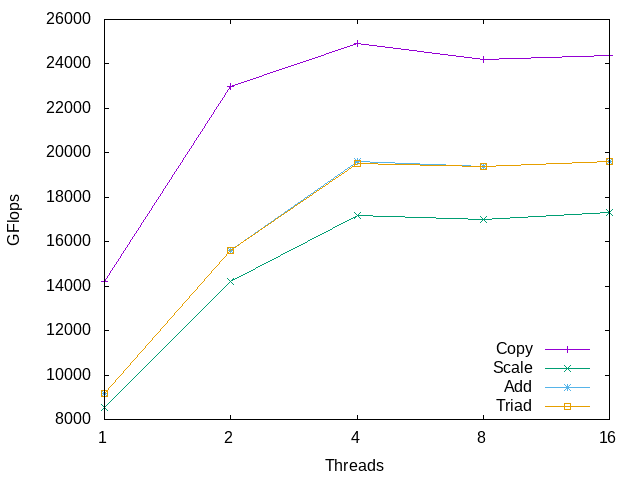
\includegraphics[width=0.5\textwidth]{img/stream_binding_one_same_grafica.png}
    \caption{Gràfica amb la performance de MB/s mitjana per diferent nombre de processos en un mateix numanode tant la memòria com els processos.}
    \label{fig:stream_binding_one_same_perf}
\end{figure}

Com veiem a la taula \ref{tab:stream_binding_diff_perf} i la gràfica \ref{fig:stream_binding_one_diff_perf}, sembla que es satura el bandwith amb 4 i 8 threads, però amb 16 millora.
% Please add the following required packages to your document preamble:
% \usepackage{multirow}
% \usepackage[table,xcdraw]{xcolor}
% If you use beamer only pass "xcolor=table" option, i.e. \documentclass[xcolor=table]{beamer}
\begin{table}[h]
    \centering
\begin{tabular}{cccc}
Processes            & Function                     & Best Rate (MB/s)                 & Avg time (s)                 \\ \hline \hline
                     & \cellcolor[HTML]{EFEFEF}Copy & \cellcolor[HTML]{EFEFEF}1.42E+04 & \cellcolor[HTML]{EFEFEF}0.07 \\
                     & Scale                        & 8.54E+03                         & 0.11                         \\
                     & \cellcolor[HTML]{EFEFEF}Add  & \cellcolor[HTML]{EFEFEF}9.20E+03 & \cellcolor[HTML]{EFEFEF}0.16 \\
\multirow{-4}{*}{1}  & Triad                        & 9.20E+03                         & 0.16                         \\ \hline
                     & \cellcolor[HTML]{EFEFEF}Copy & \cellcolor[HTML]{EFEFEF}2.87E+04 & \cellcolor[HTML]{EFEFEF}0.04 \\
                     & Scale                        & 1.73E+04                         & 0.06                         \\
                     & \cellcolor[HTML]{EFEFEF}Add  & \cellcolor[HTML]{EFEFEF}1.86E+04 & \cellcolor[HTML]{EFEFEF}0.08 \\
\multirow{-4}{*}{2}  & Triad                        & 1.86E+04                         & 0.08                         \\ \hline
                     & \cellcolor[HTML]{EFEFEF}Copy & \cellcolor[HTML]{EFEFEF}4.16E+04 & \cellcolor[HTML]{EFEFEF}0.03 \\
                     & Scale                        & 2.68E+04                         & 0.04                         \\
                     & \cellcolor[HTML]{EFEFEF}Add  & \cellcolor[HTML]{EFEFEF}2.94E+04 & \cellcolor[HTML]{EFEFEF}0.05 \\
\multirow{-4}{*}{4}  & Triad                        & 2.95E+04                         & 0.05                         \\ \hline
                     & \cellcolor[HTML]{EFEFEF}Copy & \cellcolor[HTML]{EFEFEF}4.19E+04 & \cellcolor[HTML]{EFEFEF}0.03 \\
                     & Scale                        & 3.13E+04                         & 0.03                         \\
                     & \cellcolor[HTML]{EFEFEF}Add  & \cellcolor[HTML]{EFEFEF}3.46E+04 & \cellcolor[HTML]{EFEFEF}0.05 \\ 
\multirow{-4}{*}{8}  & Triad                        & 3.49E+04                         & 0.05                         \\ \hline
                     & \cellcolor[HTML]{EFEFEF}Copy & \cellcolor[HTML]{EFEFEF}4.76E+04 & \cellcolor[HTML]{EFEFEF}0.02 \\
                     & Scale                        & 3.48E+04                         & 0.03                         \\
                     & \cellcolor[HTML]{EFEFEF}Add  & \cellcolor[HTML]{EFEFEF}3.87E+04 & \cellcolor[HTML]{EFEFEF}0.04 \\
\multirow{-4}{*}{16} & Triad                        & 3.91E+04                         & 0.04                         \\ \hline
\end{tabular}
    \caption{Performance en MB/s i temps de cada funció amb diferent nombre de processos en un diferent numanode la memòria i els processos.}
    \label{tab:stream_binding_diff_perf}
\end{table}

\begin{figure}
    \centering
    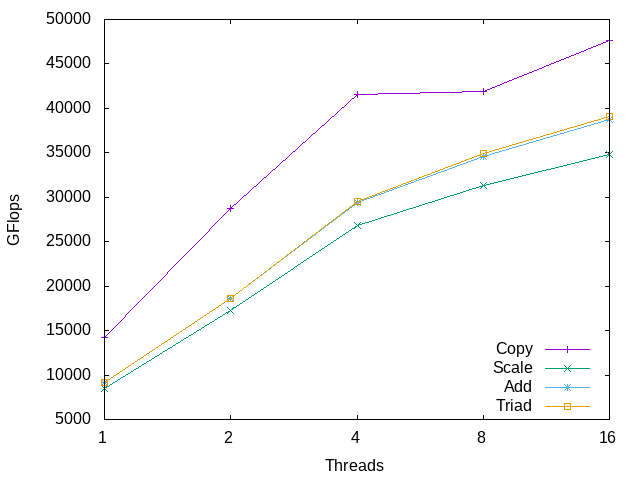
\includegraphics[width=0.5\textwidth]{img/stream_binding_one_diff_grafica.png}
    \caption{Gràfica amb la performance de MB/s mitjana per diferent nombre de processos en en diferents numanodes la memòria i els processos.}
    \label{fig:stream_binding_one_diff_perf}
\end{figure}

Com veiem a la taula \ref{tab:stream_binding_two_perf} i la gràfica \ref{fig:stream_binding_two_perf}, sembla que es satura el bandwith amb 4 i 8 threads, però amb 16 millora.
\begin{table}[h]
    \centering
\begin{tabular}{cccc}
Processes            & Function                     & Best Rate (MB/s)                 & Avg time (s)                 \\ \hline
                     & \cellcolor[HTML]{EFEFEF}Copy & \cellcolor[HTML]{EFEFEF}1.42E+04 & \cellcolor[HTML]{EFEFEF}0.07 \\
                     & Scale                        & 8.54E+03                         & 0.11                         \\
                     & \cellcolor[HTML]{EFEFEF}Add  & \cellcolor[HTML]{EFEFEF}9.19E+03 & \cellcolor[HTML]{EFEFEF}0.16 \\
\multirow{-4}{*}{1}  & Triad                        & 9.21E+03                         & 0.16                         \\ \hline
                     & \cellcolor[HTML]{EFEFEF}Copy & \cellcolor[HTML]{EFEFEF}2.73E+04 & \cellcolor[HTML]{EFEFEF}0.04 \\
                     & Scale                        & 1.69E+04                         & 0.06                         \\
                     & \cellcolor[HTML]{EFEFEF}Add  & \cellcolor[HTML]{EFEFEF}1.80E+04 & \cellcolor[HTML]{EFEFEF}0.08 \\
\multirow{-4}{*}{2}  & Triad                        & 1.80E+04                         & 0.08                         \\ \hline
                     & \cellcolor[HTML]{EFEFEF}Copy & \cellcolor[HTML]{EFEFEF}3.83E+04 & \cellcolor[HTML]{EFEFEF}0.03 \\
                     & Scale                        & 2.61E+04                         & 0.04                         \\
                     & \cellcolor[HTML]{EFEFEF}Add  & \cellcolor[HTML]{EFEFEF}2.84E+04 & \cellcolor[HTML]{EFEFEF}0.05 \\
\multirow{-4}{*}{4}  & Triad                        & 2.84E+04                         & 0.05                         \\ \hline
                     & \cellcolor[HTML]{EFEFEF}Copy & \cellcolor[HTML]{EFEFEF}3.77E+04 & \cellcolor[HTML]{EFEFEF}0.03 \\
                     & Scale                        & 2.84E+04                         & 0.04                         \\
                     & \cellcolor[HTML]{EFEFEF}Add  & \cellcolor[HTML]{EFEFEF}3.18E+04 & \cellcolor[HTML]{EFEFEF}0.05 \\
\multirow{-4}{*}{8}  & Triad                        & 3.16E+04                         & 0.05                         \\ \hline
                     & \cellcolor[HTML]{EFEFEF}Copy & \cellcolor[HTML]{EFEFEF}4.73E+04 & \cellcolor[HTML]{EFEFEF}0.02 \\
                     & Scale                        & 3.43E+04                         & 0.03                         \\
                     & \cellcolor[HTML]{EFEFEF}Add  & \cellcolor[HTML]{EFEFEF}3.83E+04 & \cellcolor[HTML]{EFEFEF}0.04 \\
\multirow{-4}{*}{16} & Triad                        & 3.86E+04                         & 0.04                         \\ \hline
\end{tabular}
    \caption{Performance en MB/s i temps de cada funció amb diferent nombre de processos en dos numanodes.}
    \label{tab:stream_binding_two_perf}
\end{table}


\begin{figure}
    \centering
    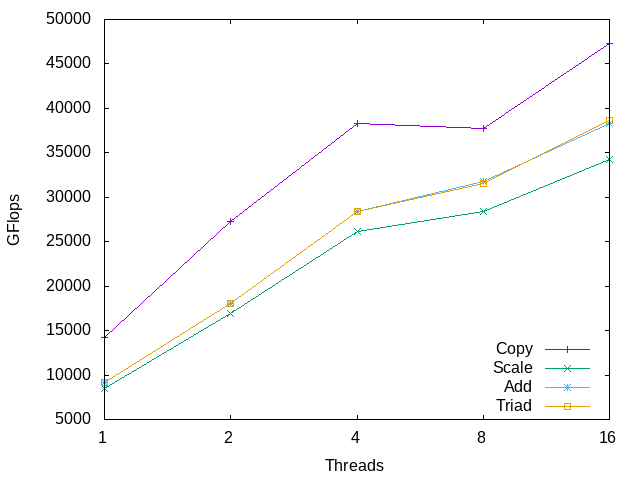
\includegraphics[width=0.5\textwidth]{img/stream_binding_two_same_grafica.png}
    \caption{Gràfica amb la performance de MB/s mitjana per diferent nombre de processos en dos numanodes.}
    \label{fig:stream_binding_two_perf}
\end{figure}
